\section{Databasestruktur}
Der er i Barteradds projektet brug for at persistere en del data, og derfor brug for en eller anden form for database, det oplagte valg var at vælge en relationel database, da der er en masse struktur SQL serveren selv holder styr på.

\subsection{Persistent data}
Ud fra domæneanalysen er det klargjort hvad det er for noget data der er nødvendigt at persistere. Der er fundet yderligere data som det er ønsket at gemme i den løbende udvikling, men som ikke er opdateret i den daværende domæneanalyse.

Det valgte data er :
\begin{itemize}
	\item BytteAnnoncer
	\begin{itemize}
		\item Beskrivelse 
		\item Billede 
		\item Kategori
		\item Kommentarer
		\item Vurdering
	\end{itemize}
	\item BrugerProfil
	\begin{itemize}
		\item Brugernavn
		\item Password
		\item E-mail
		\item Lokation
		\item BytteHistorik
		\item Rating
	\end{itemize}
\end{itemize} 

Det er vigtigt at understrege at der selvfølgelig er en række krav til disse data, der er defineret i systemarkitekturen. Brugeren skal ikke være tilgængelig for alle, og i forhold til almindelige kodeordsstandarder, skal passworded være hashet, således at applikationen ikke gemmer på nogen direkte version af kodeordet. 

\section{ER-diagram}
For at opnå større indsigt i database opbygning og problemdomænet blev der oprettet et ER-diagram for at vise sammenhængene mellem de forskellige systemklasser (Entitys) i forhold konnektivitet. Det udarbejde ER-diagram kan ses på figur \ref{fig:Erdiagram}.

\begin{figure}[H]
	\centering
	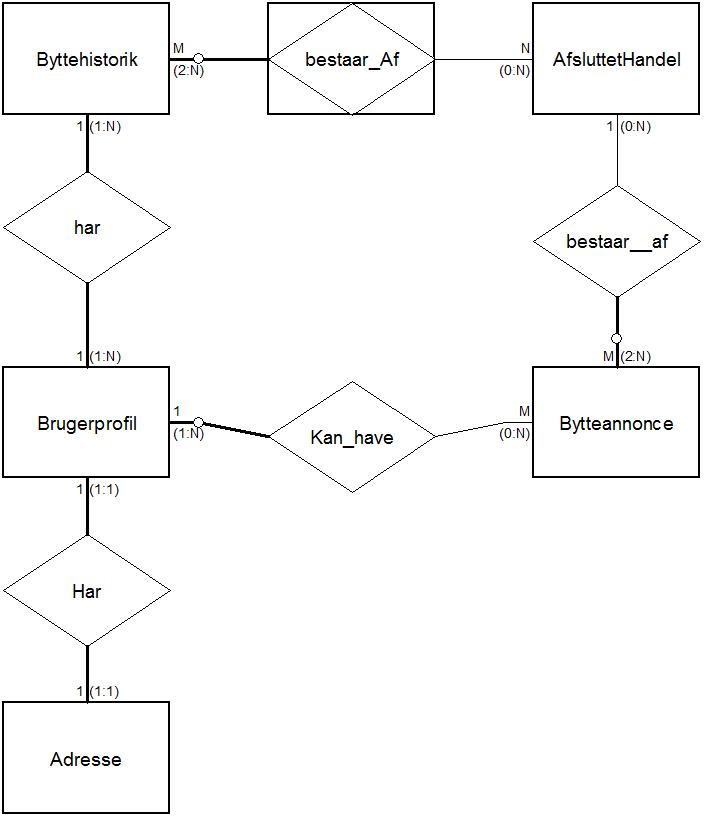
\includegraphics
	[width=165mm]
	{figures/ER-diagram.jpg}
	\caption{ER-diagram for databasen i systemet}
	\label{fig:Erdiagram}
\end{figure}


Sammen med ER-diagram blev der også udviklet en række af oneliners, der beskriver, hvordan de forskellige entities er forbundet og om et relationship er tvunget eller er mulighed.
\begin{itemize}
	\item En brugerprofil kan have mange bytteannoncer
	\item En byttannonce skal have en burgerprofil.
	\item En brugerprofil skal have en adresse.
	\item En adresse skal have en brugerprofil.
	\item En brugerprofil skal have en Byttehistorik 
	\item En byttehistorik skal have en brugerprofil
	\item En byttehistorik kan bestå af AfsluttetHandel
	\item En AfsluttetHandel skal have to Byttehistorik
	\item En AfsluttetHandel skal bestå af to Bytteannonce
	\item En Bytteannonce kan være tilknyttet en AfsluttetHandel
\end{itemize}

På baggrund af ER-diagrammet kunne databasen være designet af et genereret script. Men det blev i stedet valgt at designe databasen med en code-first database ved brug af Entity Framework.



%\subsection{DAL} 
%Databasen er i projektet lavet med entity framework, og den præcise forklaring af dette kommer i afsnit(INDSÆT!!!!). Men for selve strukturen i database overholder den ønskede systemarkitektur, hvor hvert lag ønskes både udskifteligt og testbart, er der lagt et repository pattern ned over selve databasen. Dette gør databaseteknologien yderst udskiftelig. Selve forklaringen af repository patternet kan findes i afsnit.(INSÆT!!!) Dette gør tests noget nemmere, da den resterende applikation kan testes med mocks af den unitofwork der er brugt, og er derved uafhængig af den konkrete database. Disse tests forklares i afsnit(Indsæt !!!!). Derved er Data acces laget lavet på en måde hvor det tilgås som interfaces hvor der nedenunder ligger den konkrete teknologi, hvor detaljerne i tilgangen til den relationelle database er gemt for applikationen.      
%
%\subsection{Entity Framework}
%Den konkrete teknologi der er valgt til at tilgå databasen er som nævnt entity framework. Dette er en ORM der tillader os at modellere databasen som var den objectorienteret. Frameworket er valgt da det er oplagt i sammenhæng med ASP.net, møder alle vores krav til en database og desuden er det den teknologi projektgruppen modtager undervisning i. Frameworket virker på en måde hvor den gennem de 10 database designregler opretter SQL tabeller med de tilsvarende fremmed nøgler. Derefter  opereres der på databasen via. LINQ, og selvfølgelig også stadig igennem vores repsitory pattern.      